\documentclass[9pt]{beamer}
%\documentclass[handout, 9pt]{beamer}

\usepackage{import}
\subimport{../}{preamble.tex}
\subimport{../}{beamer-theme.tex}
\usepackage{svg}

% Location for all figures / pictures
\graphicspath{{pictures/}{figures/}}

% Figures inline
\usepackage{tikz}
\usepackage{pgfplots}
\usetikzlibrary{calc}
\usetikzlibrary{shapes.multipart}
\usetikzlibrary{decorations.pathreplacing}
\usetikzlibrary{arrows.meta}
\usepgfplotslibrary{fillbetween}

\newcommand{\xbar}{1}


%--------------------------------------------------
% Presentation Information
%--------------------------------------------------
\title[Continuous Optimization]{Introduction to Continuous Optimization}
\date[]{Fall 2026}
%--------------------------------------------------

\begin{document}

\begin{frame}  

  \maketitle

  \vspace{-2em}
  
  \begin{center}
    \begin{tabular}{lll}
      Instructor : & \textbf{Bart Van Parys} & \textbf{(\href{mailto:mastermath@vanparys.xyz}{mastermath@vanparys.xyz})} \\
    \end{tabular}
  \end{center}
  
\end{frame}

\section{History}

\begin{frame}{Nature As Optimizer : Fermat's Principle}

  Fermat : ``Light takes the fastest optimal path (in hindsight)'' 
  
  \begin{center}
    \includesvg[height=4cm]{snell.svg}
  \end{center}

  \uncover<2->{
  Travel time:
  \[
    f(x) = \frac{\sqrt{x^2+a^2}}{c/n_1} + \frac{\sqrt{b^2 + (l-x)^2}}{c/n_2}
  \]

  \begin{itemize}
  \item The actual observed $x^\star$ will be a minimizer of $f(x)$
  \item Is equivalent to Snell's law: $n_1\sin(\theta_1)=n_2\sin(\theta_2)$
  \end{itemize}
  }
\end{frame}

\begin{frame}{History of Optimization -- Univariate Problems}

  \begin{center}
    \includegraphics[height=4cm]{univariate-function/univariate-function.pdf}
  \end{center}
  
  \begin{itemize}
  \item Fermat, 1638 and Newton, 1670
    $$ x^\star \in \arg \min \; f(x)\qquad \mbox{$x$: scalar} $$

    Necessary condition : $$ f'(x^\star)=0 $$

  \end{itemize}
\end{frame}

\begin{frame}{History of Optimization -- Multivariate Problems}

  \begin{center}
    \includegraphics[height=4cm]{rosenbrock/rosenbrock.pdf}
  \end{center}
  
  \begin{itemize}
  \item Euler, 1755 
    $$  \min \; f(x_1, \ldots, x_n)  $$
    Necessary condition : $$ \nabla f({x}^\star)=0   $$  
  \end{itemize}
\end{frame}


\begin{frame}{History of Optimization -- Constraint Problems}

  Constraint mechanics
  \begin{center}
    \includesvg[height=2.5cm]{lagrangian-mechanics.svg}
  \end{center}

  \begin{itemize}
  \item Lagrange, 1797: ``M\'ecanique Analytique''

    \[
      \begin{array}{rl}
        \min & f(x_1, \ldots, x_n)\\[0.5em]
        \st & \forall k=1,\ldots,m:\\
            & \quad  g_k(x_1, \ldots, x_n)=0.
      \end{array}
    \]
  \item Method of Lagrange multipliers (See duality theory!)
  \end{itemize}
\end{frame}

\begin{frame}{History of Optimization -- Calculus of Variations}

  Which slide is the fastest? (Johann Bernoulli 1696)
  \begin{center}
    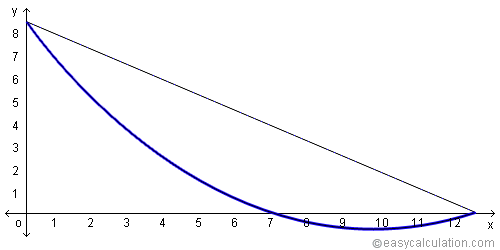
\includegraphics[height=3cm]{brachistochrone_curve.png}
  \end{center}
  \begin{itemize}
  \item Brachistochrone (``Shortest time'')
  \end{itemize}
  
    \hfill
  \begin{itemize}
  \item Euler, Lagrange : Calculus of variations. 
  \end{itemize}

\end{frame}

\begin{frame}{Huygens's Optimal Pendulum}

  Is there a pendulum whose frequency is independent of its amplitude?
  \begin{center}
    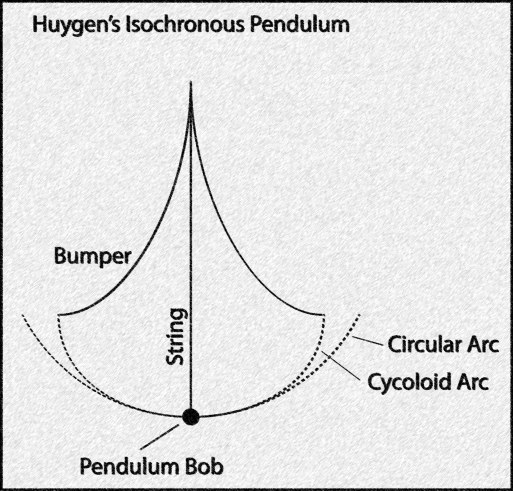
\includegraphics[height=5cm]{tautochrone_curve.jpg}
  \end{center}
  \begin{itemize}
  \item Tautochrone (``Equal time'')
  \end{itemize}
  
    \hfill
  \begin{itemize}
  \item<2-> Huygens' implementation was a failure\dots
  \end{itemize}

\end{frame}

\section{Least Squares Optimization}

\begin{frame}{Least Squares Regression}

  Supervised Data
  \begin{itemize}
  \item \makebox[3.225cm]{Covariates : \hfill} $X \defn (x_1, \dots, x_n) \in \Re^{n\times p}$
  \item \makebox[3.225cm]{Labels : \hfill} $Y \defn (y_1, \dots, y_n) \in \Re^n$
  \end{itemize}
  \vspace{1em}
  \makebox[3.9cm]{\hfill} $Y \approx X \mathbf{\blue{w}}$
  \vspace{0.5em}
  
  \textbf{Least Squares Regression :}
  \vfill
  \begin{equation*}
    \begin{array}{rl}
      w^\star \in \arg \min_{w\in\Re^p} & \sum_{i=1}^n (y_i - x_i\tpose w)^2
    \end{array}
  \end{equation*}
  \vfill

  
  \begin{minipage}{0.65\textwidth}
    \textit{Math history :}
    \begin{itemize}
    \item<2-> \textit{Legendre (1805) : Least-squares method}\\
    \item<3-> \textit{Gau\ss~(1809) : Celestial mechanics of Ceres}\\
    \item<3-> Big data in 1809: $n=22$!
    \end{itemize}
  \end{minipage}%
  \hfill
  \begin{minipage}{0.35\textwidth}
    \uncover<2->{%
    \begin{minipage}{0.5\textwidth}
      \centering
      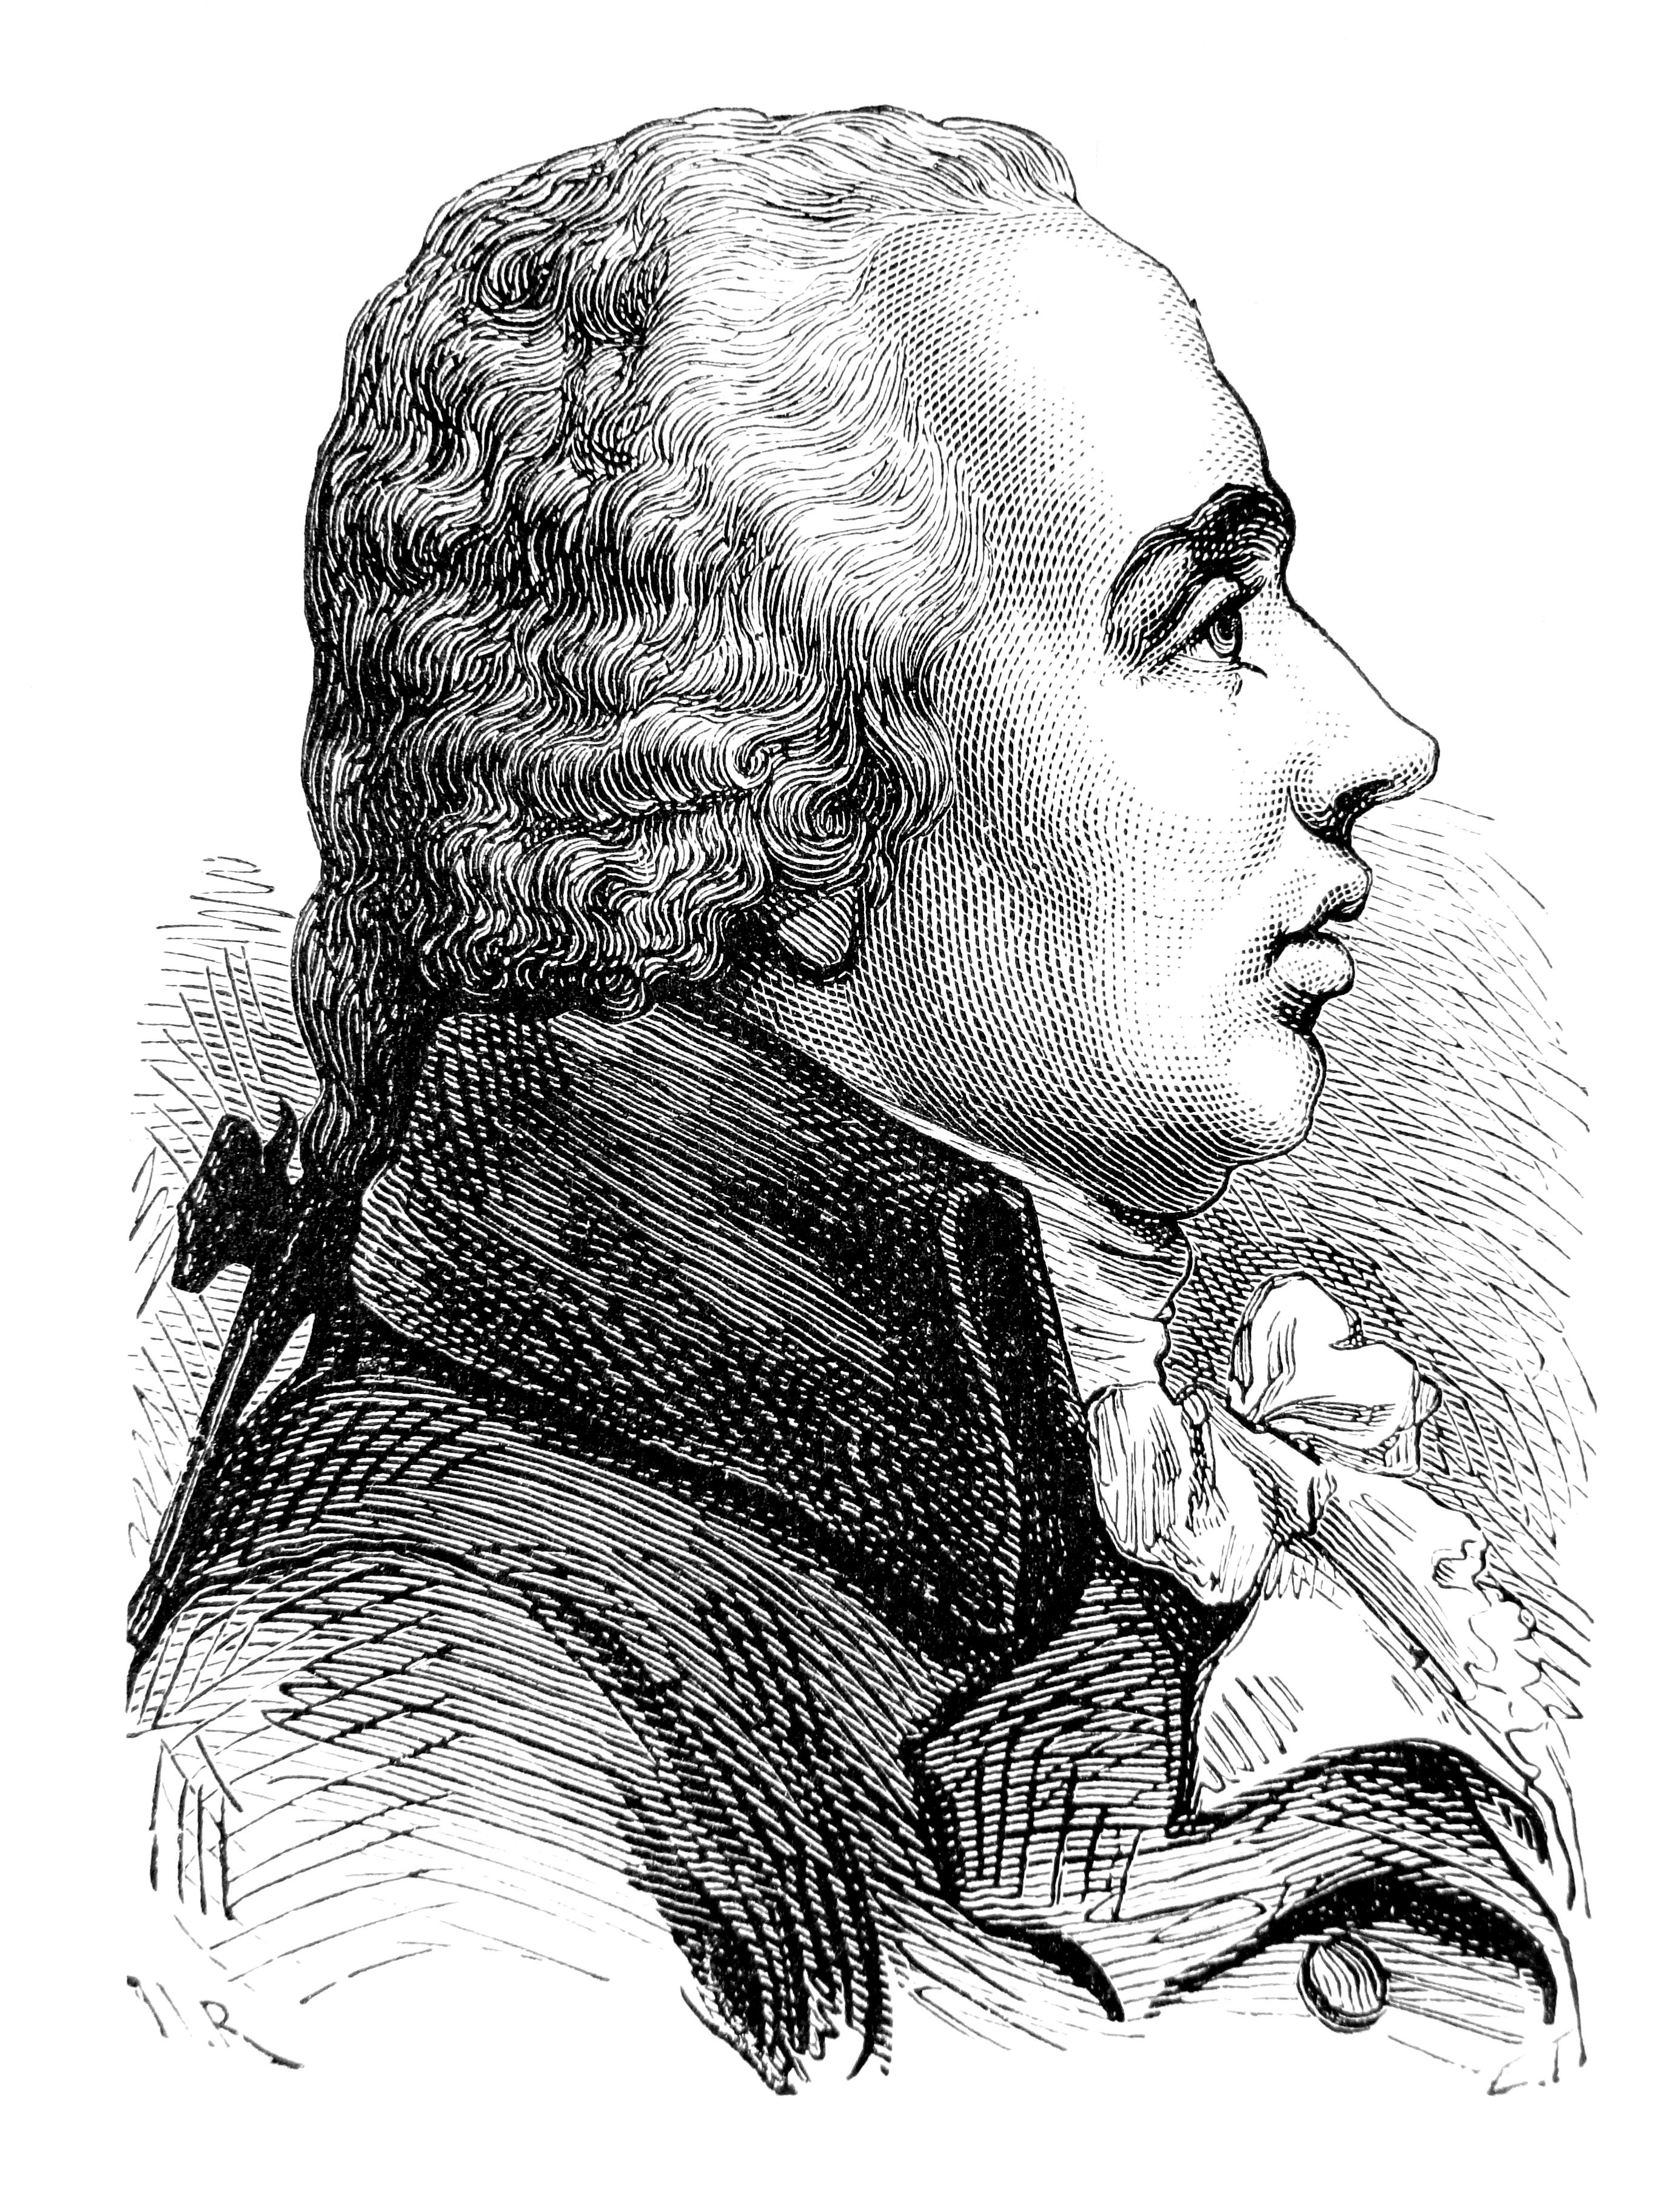
\includegraphics[height=2.5cm]{young-legendre.jpg}\\
      Legendre
    \end{minipage}%
    }%
    \hfill
    \uncover<3->{%
    \begin{minipage}{0.5\textwidth}
      \centering
      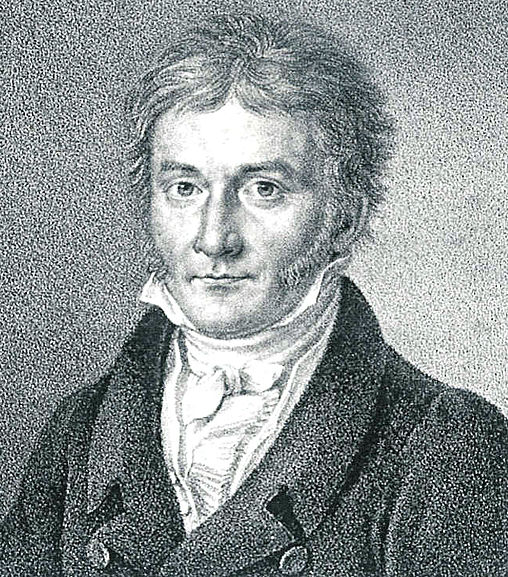
\includegraphics[height=2.5cm]{young-gauss.jpg}\\
      Gau\ss
    \end{minipage}
    }%
  \end{minipage}

  \vfill

\end{frame}

\begin{frame}{Least Squares Optimization}

  \begin{minipage}{1\textwidth}
    Least Squares Matrix Notation :
    \vfill
    \begin{equation*}
      \begin{array}{rl}
        \minimize & \norm{Y - X w}^2_2\\[0.5em]
        \st & w\in\Re^p
      \end{array}
    \end{equation*}
  \end{minipage}%
  % \hfill
  % \begin{minipage}{0.4\textwidth}
  %   \centering
  %   \includegraphics[height=3.5cm]{least-squares/least-squares.pdf}
  % \end{minipage}
  \vfill

  \textbf{Quadratic Optimization Problem :}
  \begin{itemize}
  \item Analytical solution as a linear equation
    \[
      (X\tpose X)\,w^\star = X\tpose Y
    \]

  \item Reliable and efficient algorithms and software
  \item Computational time scales as $n^2 p$ ($X\in\Re^{n\times p})$
  \item<2-> Mature technology
  \end{itemize}
  
\end{frame}

\section{Linear Optimization}

\begin{frame}{Linear Optimization}

  \begin{minipage}{0.5\textwidth}
    \textbf{Linear Optimization :}\\[0.5em]
    \begin{equation*}
      \begin{array}{rl}
        \minimize & c\tpose x \\[0.5em]        
        \st & x\in\Re^n \\[0.5em]
        & a_i\tpose x \leq b_i, \quad \forall i \in [1, \dots, k]
      \end{array}
    \end{equation*}
  \end{minipage}%
  \begin{minipage}{0.5\textwidth}
    \centering
    \includegraphics[height=3.5cm]{linear-optimization/linear-optimization.pdf}
  \end{minipage}

  \vfill
  
  \begin{minipage}{0.6\textwidth}    
    \textbf{Properties :}
    \begin{itemize}
    \item No analytical solution
    \item Reliable and efficient algorithms and software
    \item Computational time scales as $n^2 k$
    \item<2-> Mature technology
    \end{itemize}
  \end{minipage}%
  \hfill
  \begin{minipage}{0.2\textwidth}
    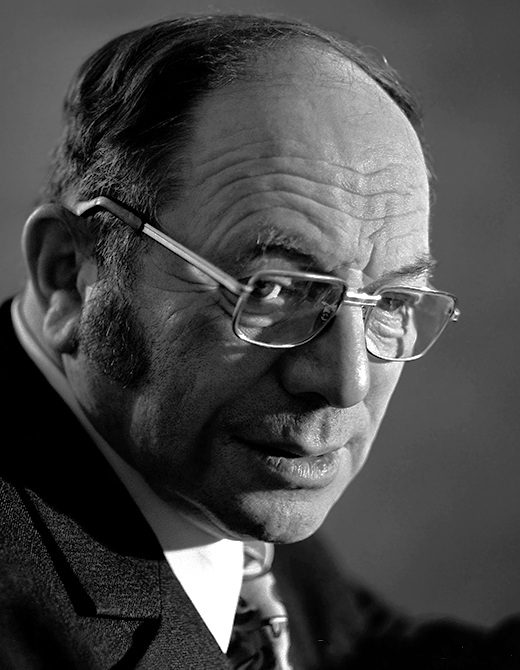
\includegraphics[height=2.5cm]{kantorovich.jpg}\\
    Kantorovich
  \end{minipage}%
  \begin{minipage}{0.2\textwidth}
    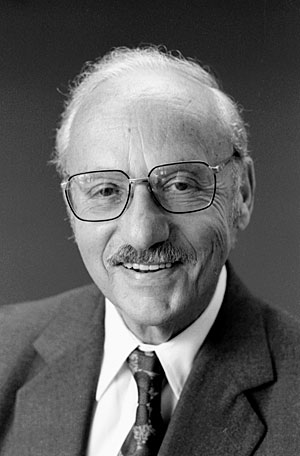
\includegraphics[height=2.5cm]{dantzig.jpg}\\
    Dantzig
  \end{minipage}

\end{frame}

\begin{frame}{Transport Logistics}

  We have $n$ consumers requiring a \emph{demand} $d_1, \dots, d_n$ of product. Every consumer needs to be serviced by any of $m$ distribution facilities stocking a \emph{supply} $s_1, \dots, s_m$. The \emph{marginal cost} of shipping from supply facility $j$ to consumer $i$ is denoted as $c_{ij}$.


  \begin{center}
    \includegraphics[height=3.5cm]{transport/transport.pdf}
  \end{center}
  
  Define : $x_{ij}$ as the \emph{amount supplied} from the $j$-th facility to the $i$-th consumer.
  
  \vfill

  \uncover<2->{
  \[
    \begin{array}{rl}
      \minimize & \sum_{i=1}^n \sum_{j=1}^m c_{ij} x_{ij} \\[0.5em]
      \st & x_{ij} \geq 0 \quad i\in [1, \dots, n], ~j\in [1, \dots, m] \\[0.5em]
                & \sum_{i=1}^n x_{ij} \leq s_j\quad j\in [1, \dots, m] \\[0.5em]
                & \sum_{j=1}^m x_{ij} \geq d_i\quad i\in [1, \dots, n]
    \end{array}
  \]
  }
  
\end{frame}

\begin{frame}{Who's Who in Mathematics}

  \begin{minipage}{0.16\textwidth}
    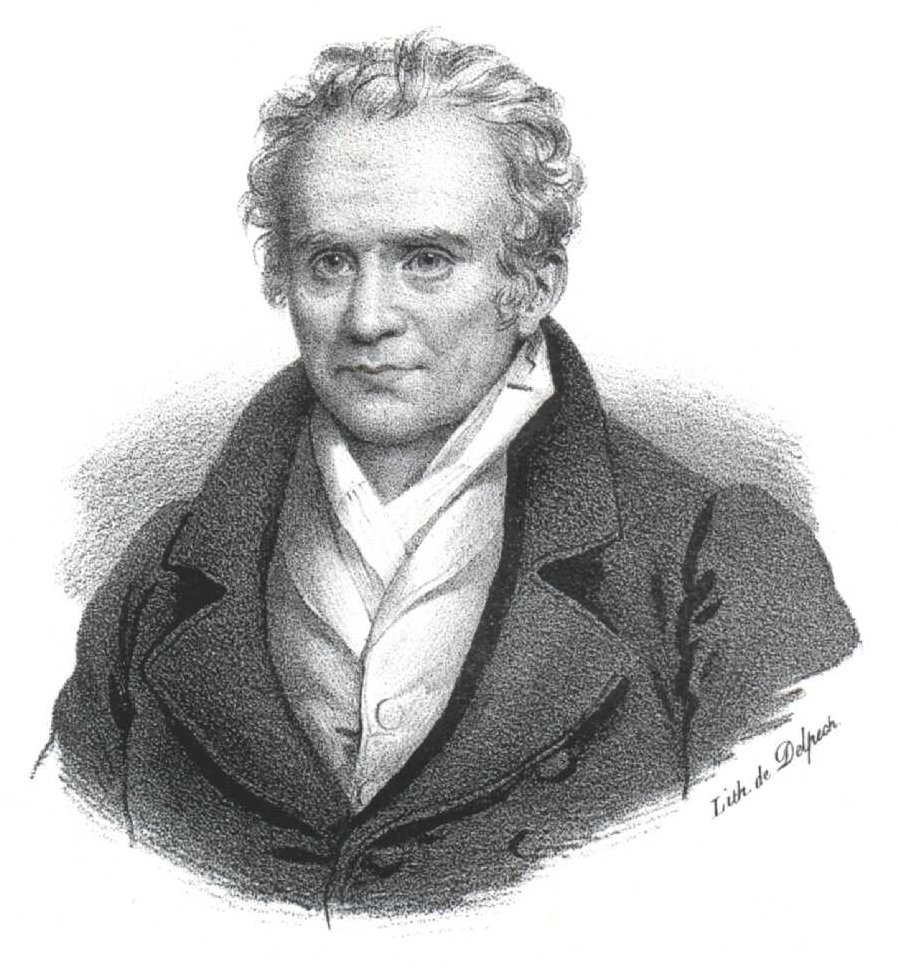
\includegraphics[height=2.5cm]{monge.jpg}
  \end{minipage}%
  \hfill
  \begin{minipage}{0.16\textwidth}
    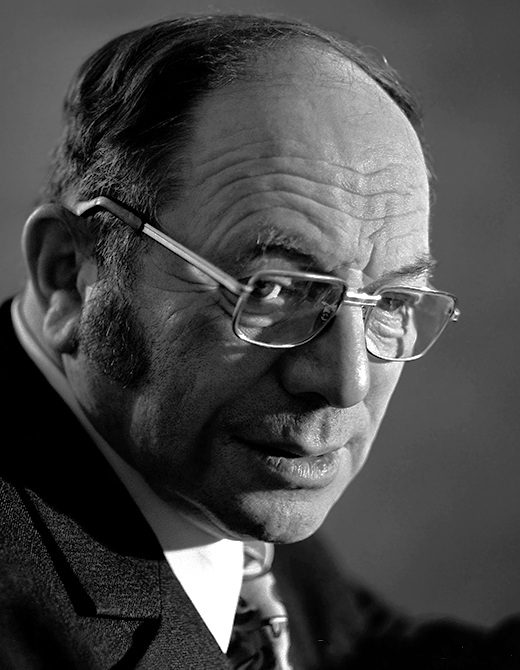
\includegraphics[height=2.5cm]{kantorovich.jpg}
  \end{minipage}%
  \hfill
  \begin{minipage}{0.16\textwidth}
    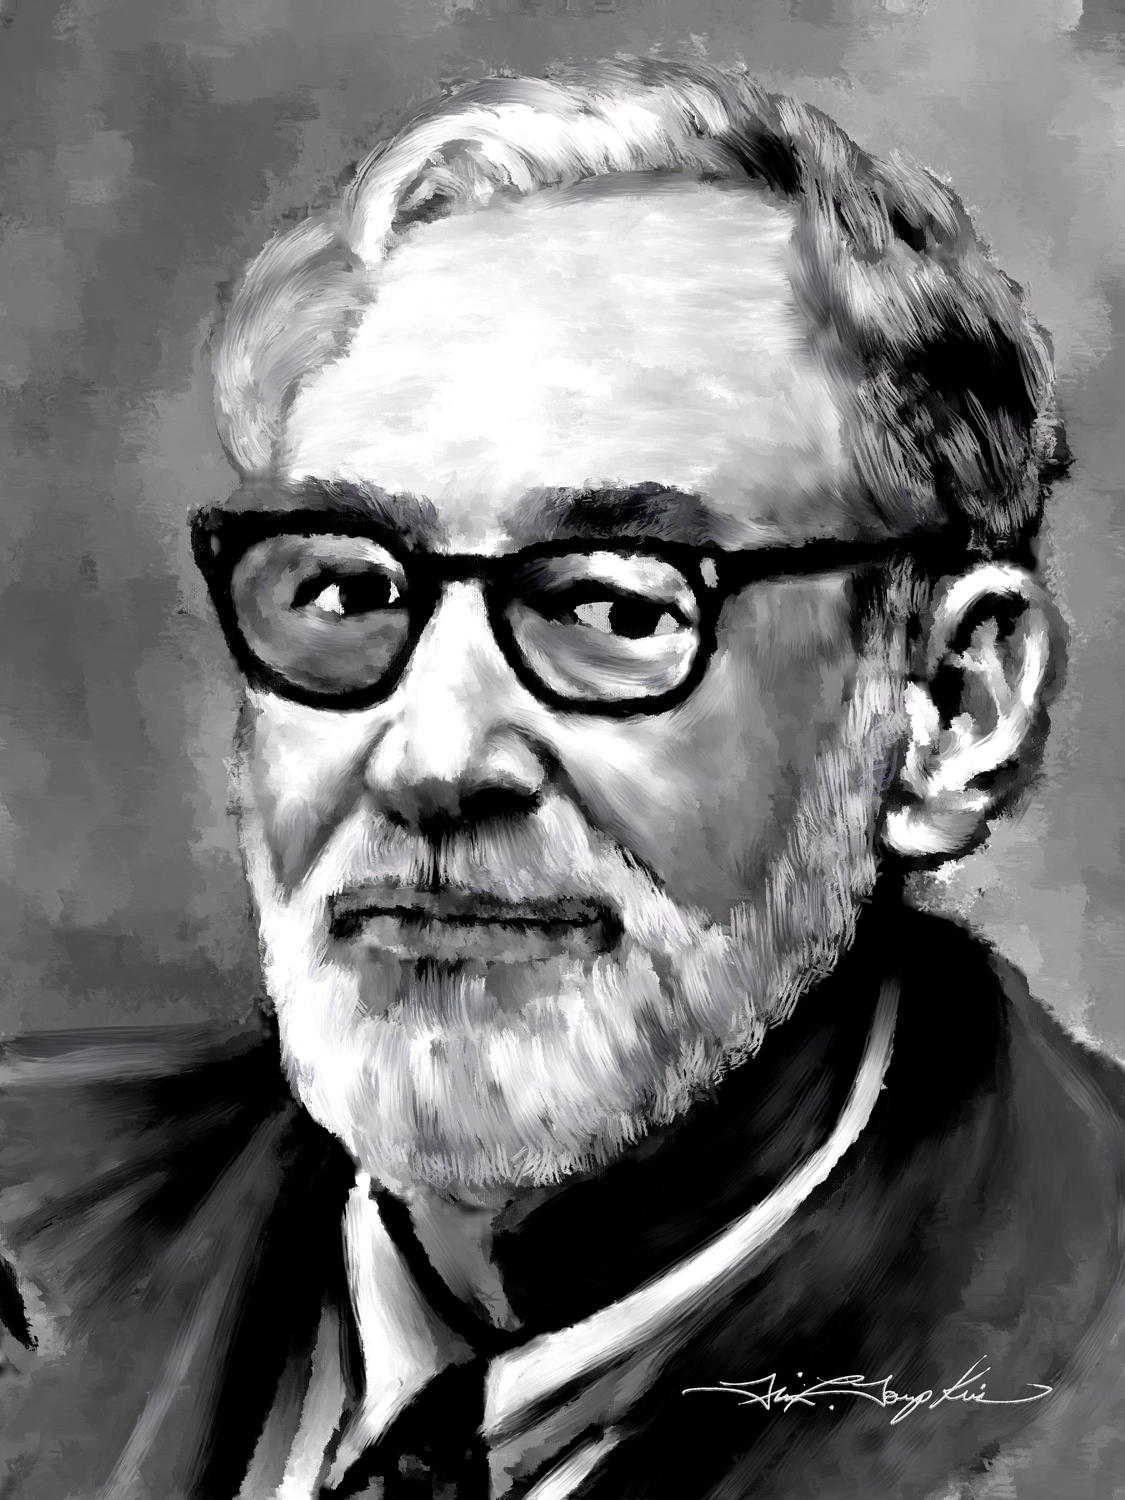
\includegraphics[height=2.5cm]{koopmans.jpg}
  \end{minipage}%
  \hfill
  \begin{minipage}{0.16\textwidth}
    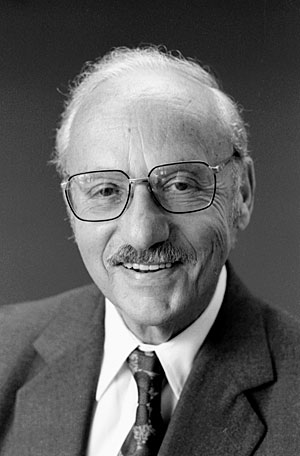
\includegraphics[height=2.5cm]{dantzig.jpg}
  \end{minipage}%
  \hfill
  \begin{minipage}{0.16\textwidth}
    
\includegraphics[height=2.5cm]{villani.jpg}
  \end{minipage}%
  \hfill
  \begin{minipage}{0.16\textwidth}
    
\includegraphics[height=2.5cm]{figalli.jpg}
  \end{minipage}%
  
  
  
  
  \vfill
  
  From left to right
  \begin{enumerate}
  \item Gaspard Monge: ``Sur la th\'eorie des déblais et des remblais''
  \item Leonid Kantorovich: Formulation as (infinite dimensional) linear optimization
  \item Tjalling Koopmans \& Leonid Kantorovich: Nobel prize for economic planning
  \item George Dantzig: Simplex method
  \item C\'edric Villani : Fields medal
  \item Alessio Figalli: Fields medal
  \end{enumerate}
  
\end{frame}

\begin{frame}{Statistical Risk -- Problem}

  \emph{Example} : Suppose revenue $R$ is distributed on $n$ equidistant points $r_i$ on the interval $\Omega = [-10, 100]$.
  We assume the following prior information
  \begin{itemize}
  \item Mean : $\E{}{R} \in [15, 20]$
  \item Second-order moment : $\E{}{R^2} \in [500,600]$
  \item Higher-order information : $\E{}{3 R^3-2 R} =40000$ 
  \end{itemize}

  \vfill

  \emph{Problem:} What is the worst probability of loss $\mb P(R<0)$?

\end{frame}

\begin{frame}{Statistical Risk -- Solution}
  
  Decision variable : $p_i \defn \mb P(R=r_i)$.
  
  \vfill
  
  \begin{equation*}
    \begin{array}{rl}
      {\displaystyle\max_{p}} & \sum_{\set{i\in[1, \dots, n]}{r_i < 0}} p_i \\[0.5em]
      \st & p\geq 0, ~\sum_{i=1}^n p_i = 1,\\[0.5em]
           &  15 \leq \sum_{i=1}^n r_i p_i \leq 20,\\[0.5em]
                & 500 \leq \sum_{i=1}^n r^2_i p_i \leq 600,\\[0.5em]
                & \sum_{i=1}^n \left( 3 r^3_i - 2r_i\right) p_i = 40000.
    \end{array}
  \end{equation*}

  \vfill

  \begin{itemize}
  \item Solution : see provided Julia program.
  \end{itemize}
  
\end{frame}



\section{Nonlinear Optimization}

\begin{frame}{Optimization}
  Optimization is about making good \emph{decisions} in a \emph{disciplined} way, often subject to constraints. Applications appear everywhere in science, mathematics and business:

  \vfill
  
  \begin{itemize}
  \item Managing a portfolio
  \item Scheduling public transport
  \item Fitting a model to measured data
  \item Optimizing a supply chain
  \item Designing electronic circuits
  \item Choosing worker shift patterns
  \item Shaping aerodynamic components
  \item Recovering images from raw MRI data
  \end{itemize}

\end{frame}


\begin{frame}{Describing an Optimization Problem}

  \textbf{Optimization Problem :}

  \vfill
  \[
    \begin{array}{rl}
      \minimize & f(x) \\[0.5em]
      \st & x \in E, \\[0.5em]
                & x\in X \subseteq E.
    \end{array}
  \]

  \vfill

  An optimization problem of several parts
  \begin{itemize}
  \item The vector $x$ collects the \emph{optimization variables}
  \item The linear space $E(=\Re^n, \Re^{n\times n})$ is the \emph{domain} of the decision variables
  \item The set $X$ is the \emph{constraint set}, and describes the \emph{feasible decisions}
  \item The \emph{objective} function $f:E\to\Re$ assigns cost $f(x)$
  \end{itemize}

\end{frame}

\begin{frame}{Potential Problems}

  \begin{enumerate}
  \item Example:
    \[
      \begin{array}{rl}
        \minimize & \exp{(x)} \\
        \st  & x\leq -1 \\
                  & x \geq 0
      \end{array}
    \]

  \item<2-> If the constraints are inconsistent, then the problem is \emph{infeasible}.
  \item<3-> Example:
    \[
      \begin{array}{rl}
        \minimize & x \\
        \st   & x\leq 0 \\
      \end{array}
    \]    
  \item<4-> It might be possible that the problem is \emph{unbounded}.
  \item<5-> Example:
    \[
      \begin{array}{rl}
        \minimize & \exp{(x)}
      \end{array}
    \]
  \item<6-> Problem can be feasible and bounded, but no optimal solution exists.
  \end{enumerate}
  
\end{frame}


\begin{frame}{Terminology}

  \emph{Solving} the \emph{Nonlinear Optimization} problem :
  \[
    \begin{array}{rl}
      \minimize & f(x) \\[0.5em]
      \st & x \in E, \\[0.5em]
                & x\in X \subseteq E,
    \end{array}
  \]
  requires determining
  \begin{itemize}
  \item<2-> If the set $X$ is empty, then the problem is \emph{infeasible} ($J^\star=\infty$)
    
  \item<3-> If $J^\star = -\infty$, then the problem is \emph{unbounded below}
  \item<4-> the infimum (greatest lower bound)
    \[
      \begin{array}{rl}
        J^\star = \inf_x & f(x) \\
        \st & x\in X \subseteq E
      \end{array}
    \]
  \item<5-> the set of minimizers
     \(
      \arg \min_{x\in X} f(x) \defn \set{x\in X\subseteq E}{f(x)\leq J^\star}
    \)
  \item<5-> the set of $\epsilon$-suboptimal solutions
    \(
      \arg \min_{x\in X} f(x) \defn \set{x\in X\subseteq E}{f(x)\leq J^\star\red{+\epsilon}}
    \)
  \end{itemize}
  
\end{frame}



\begin{frame}{Nonlinear Optimization Problem}

  \textbf{More common problem formulation :}

  \vfill
  \[
    \begin{array}{rl}
      \minimize & f(x) \\[0.5em]
      \st    & {x\in E} \\[0.5em]
             & g_i(x) \leq 0 \quad \forall i \in [1, \dots, m]\\[0.5em]
             & h_i(x) = 0 \quad \forall i \in [1, \dots, \ell]
    \end{array}
  \]
  \vfill
  
  Defined by the problem data :
  \begin{itemize}
  \item \emph{Objective function} $f:E\to\Re$
  \item \emph{Domain} $E$ of the objective function 
  \item \emph{Inequality constraint functions} $g_i : E\to\Re$ for $i$ in $[1, \dots, m]$
  \item \emph{Equality constraint functions} $h_i : E\to\Re$ for $i$ in $[1,\dots, \ell]$
  \item \emph{Feasible set}
    \[
      X = \set{x\in E}{g_i(x) \leq 0 ~~\forall i \in [1, \dots, m],~h_i(x) = 0 ~~ \forall i \in [1, \dots, \ell] }
    \]
  \end{itemize}
  
  
\end{frame}

\begin{frame}{Nonlinear Optimization Problem : Example}

  \begin{minipage}{0.55\textwidth}

    \textbf{Problem :} In $\Re^2$, find the point in the unit box $X$ closest to the point $(x_1, x_2) = (3, 2)$.

    \vspace{3cm}
    
  \end{minipage}%
  \hfill
  \begin{minipage}{0.45\textwidth}
    \centering
    \includegraphics[height=4cm]{constraint-optimization/constraint-optimization.pdf}
  \end{minipage}

  \vfill
  
  \textbf{Standard Form}

  \begin{equation*}
    \begin{array}{rl}
      \minimize & (x_1-3)^2+(x_2-2)^2 \\[0.5em]
      \st & (x_1, x_2) \in \Re^2, \\[0.5em]
                & x_1 \leq 1, ~-x_1 \leq 1,\\[0.5em]
                & x_2 \leq 1, ~-x_2 \leq 1.
    \end{array}
  \end{equation*}
  
\end{frame}

\begin{frame}{Terminology}

  Nonlinear optimization problem :
  \vfill
  \[
  \begin{array}{rl}
    J^\star = \inf & f(x) \\[0.5em]
    \st    & x\in E\\[0.5em]
           & g_i(x) \leq 0, \quad \forall i \in [1, \dots, m]\\[0.5em]
                     & h_i(x) = 0, \quad \forall i \in [1, \dots, \ell]
  \end{array}
  \]
  \vfill
  
  \begin{itemize}
  \item \emph{Feasible point} : A point $x$ in $E$ satisfying the inequality and equality constraints, i.e., $g_i(x)\leq 0$ for $i$ in $[1, \dots, m]$ and $h_i(x)=0$ for $i$ in $[1, \dots, \ell]$.

  \item \emph{Strictly feasible point} : A feasible point $x$ in $E$ satisfying the inequality constraints strictly, i.e., $g_i(x)<0$ for $i$ in $[1, \dots, m]$.

  \item A \emph{redundant constraint} does not influence the feasible set.

    \[
      \begin{array}{rl}
        \min_{x\in\Re} & f(x) \\
        \st & x\leq 1 \\
                       & x\leq 3 \quad \emph{redundant}
      \end{array}
    \]
  \end{itemize}
  
\end{frame}

\begin{frame}{Solution Types}

  \[
    \begin{array}{rl}
      \minimize & f(x) \\[0.5em]
      \st & x\in E,\\[0.5em]
          & x\in X \subseteq E.
    \end{array}
  \]

  \vfill
    
  Solution Types:
  \begin{itemize}
  \item \emph{Global minimizer} : Any feasible $x^\star$ in $X$ such that $f(x^\star) \leq f(x)$ for all feasible $x\in X$.
    \vspace{0.5em}
  \item \emph{Local minimizer} : Any feasible $x^\star$ in $X$ such that $f(x^\star) \leq f(x)$ for all $x\in X \cap B(x^\star, \epsilon)$ for some ball $B(x^\star, \epsilon) \defn \set{x\in E}{\norm{x-x^\star}<\epsilon}$.
  \end{itemize}
  
\end{frame}

\begin{frame}{Geometry of an Optimization Problem}

  \centering
  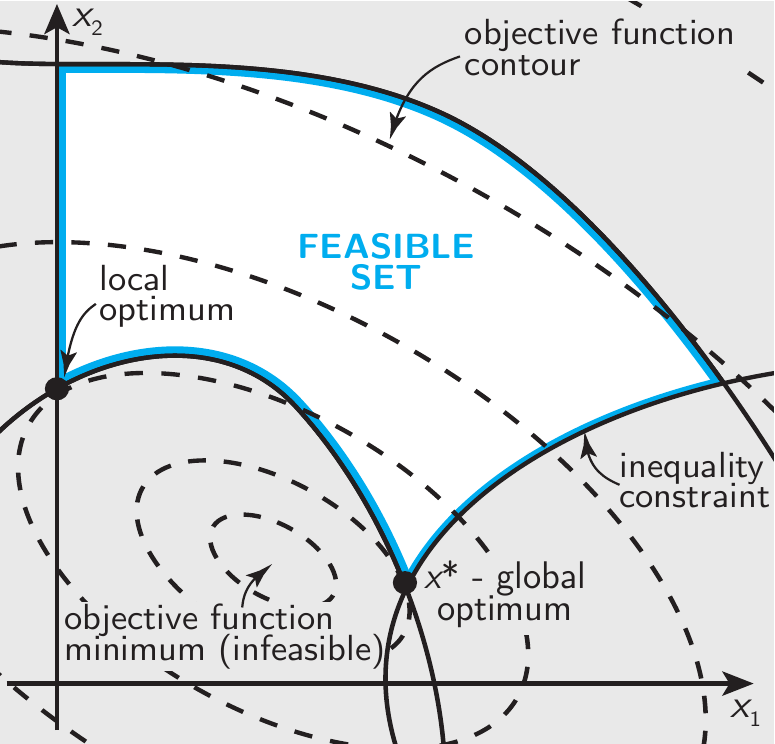
\includegraphics[width=0.65\textwidth]{geometry.png}

\end{frame}

\section{Convex Optimization}

\begin{frame}{Convex Optimization}


  \begin{minipage}{0.55\textwidth}
    \textbf{Important Special Case :}
    \[
      \begin{array}{rl}
        \minimize & f(x) \\[0.5em]
        \st    & x\in E\\[0.5em]
                  & g_i(x) \leq 0, \quad \forall i \in [1, \dots, m],
      \end{array}
    \]
    
    where the objective and constraint functions are \emph{convex functions}.
  \end{minipage}%
  \hfill
  \begin{minipage}{0.45\textwidth}
    
    \begin{center}
      \includegraphics[height=4.5cm]{convex-function/convex-function.pdf}
    \end{center}
    
  \end{minipage}

  \vfill
  A function $f$ is convex when
  \[
    \forall x, y\in E, ~\forall \theta \in [0, 1] : \quad f(\theta\cdot x+(1-\theta)\cdot y) \leq \theta\cdot f(x) + (1-\theta)\cdot f(y).
  \]
  \vfill

  \begin{itemize}  
  \item Includes least-squares and linear optimization as special cases
  \end{itemize}

\end{frame}

\begin{frame}{Brief History of Convex Optimization}

  \textbf{Theory (convex analysis)} : ca 1900--1970
  \vfill
  \textbf{Applications}
  \begin{itemize}
  \item before 1990: mostly in operations research; few in engineering
  \item since 1990: many new applications in engineering (control, signal processing, communications, \dots); new problem classes (semi-definite optimization, robust optimization)
  \end{itemize}
  \vfill
  \textbf{Algorithms}
  \begin{itemize}
  \item 1947: Simplex algorithm for linear programming (Dantzig)
  \item 1960s: Early interior-point methods (Fiacco \& McCormick, Dikin, \dots)
  \item 1970s: Ellipsoid method and other subgradient methods
  \item 1984: Polynomial-time interior-point method for linear programming (Karmarkar)
  \item 1990s--2010s: Polynomial-time interior-point methods for nonlinear convex optimization (Nesterov \& Nemirovski)
  \item 2010s--now: Large-scale first-order methods (stochastic gradient, accelerated methods)
  \end{itemize}
  
\end{frame}


\begin{frame}{Course Overview}

  \textbf{Introduction}
  \begin{enumerate}
  \item Convex Sets
  \item Convex functions
  \end{enumerate}

  \vfill
  
  \textbf{Theory}
  \begin{enumerate}
  \item Duality
  \item Conjugate Functions
  \item KKT
  \end{enumerate}

  \vfill

  \textbf{Algorithms}
  \begin{enumerate}
  \item Black Box Methods
  \item Gradient Method
  \item Newton Method
  \item Interior Point Methods
  \item SGD
  \end{enumerate}
  
\end{frame}



% ===== Convex-set recap (imported from Lecture 2) =====
\section{Convex Sets}

\begin{frame}{Linear Sets}

  A set $L \subseteq E$ is \emph{linear} if $x, y \in L$ implies
  \[
    a x + b y \in L,
  \]
  for any $a, b \in \Re$.

  \vfill
  \begin{center}
    \includesvg[height=3cm]{linear-subspace.svg}
  \end{center}
  \vfill

  \textbf{Examples :}
  \begin{itemize}
  \item Linear spaces such as $\Re^n$, $\Re^{n\times m}$
  \item Symmetric matrices $S^n\defn \set{X\in\Re^{n\times n}}{X=X\tpose}$
  \item<2-> Null space $\set{x\in\Re^m}{Ax=0}$ of a matrix $A\in\Re^{n\times m}$ 
  \end{itemize}
  
\end{frame}

\begin{frame}{Linear Hull}

  The \emph{linear hull} $span (S) \defn \cap_{L~\rm{linear},\, S\subseteq L} ~L$ of a set $S$ is the unique smallest linear set that contains $S$, i.e.\
  $$ L~\mathrm{linear~set}, ~S \subseteq L \implies span(S) \subseteq L$$  

  \vfill

  The \emph{dimension} $\dim(L)=k$ of a linear space $L$ is the smallest number of vectors $v_i\in L$ such that $$span(\{v_1, \dots, v_k\}) = L.$$

  \vfill
  
  Example:
  \begin{itemize}
  \item Symmetric matrices: $\dim(S^n) = (n+1)n/2$
  \end{itemize}
  
\end{frame}

\begin{frame}{Affine Sets}

    
  A set $H \subseteq E$ is \emph{affine} if $x, y \in H$, $\theta \in \Re$ implies
  \[
    \theta x + (1-\theta) y \in H.
  \]    

  \vfill
  \begin{center}
    \includegraphics[height=1.5cm]{affine-set/affine-set.pdf}
  \end{center}
  \vfill

  
  \textbf{Examples :}

  \begin{itemize}
  \item Linear spaces are affine
  \item Solution set of linear system $\set{x\in\Re^m}{Ax = b}$ with $A\in \Re^{m\times n}$
  \end{itemize}

  \vfill

  \uncover<2->{
  If $H$ is an affine set, then $\set{x-x_0}{x\in H}$ with $x_0\in H$ is a \emph{linear subspace}.\\[0.5em]
  The \emph{dimension} $\dim(H)$ of an affine set is the dimension of its associated subspace.
  }
\end{frame}

\begin{frame}{Affine Hull}

  The \emph{affine hull} $\aff (S) \defn \cap_{H~\rm{affine},\, S\subseteq H} ~H$ of a set $S$ is the unique smallest affine set that contains $S$, i.e.\
  $$ H~\mathrm{affine~set}, ~S \subseteq H \implies \aff(S) \subseteq H$$  

  \vfill
  \begin{minipage}{1\textwidth}
    \begin{center}
      \includegraphics[height=4cm]{affine-hull/affine-hull.pdf}
    \end{center}
  \end{minipage}
  \vfill
  
  \uncover<2->{The \emph{affine dimension} $\dim(S)$ of a set $S$ is the dimension of $\aff(S)$ (nonstandard)}

\end{frame}

\begin{frame}{Quiz}

\end{frame}

\begin{frame}{Affine Combinations}

  Consider a finite set of points $x_i$ for $i$ in $I=[1, \dots, k]$. An \emph{affine combination} is any point of the form
  \[
    \sum_{i\in I} p_i \cdot x_i
  \]
  where $p_i\in\Re$ and $\sum_{i\in I} p_i=1$.

  \vfill
  
  \textbf{Theorem : } An affine set $H \subseteq E$ is closed under affine combinations.

  \vfill
  
  \textbf{Theorem : } The affine hull of a set $S$ can be found as
  \[
    \aff (S) = \set{\sum_{i\in I} p_i\cdot x_i}{\forall k\in \N, ~\forall i\in I=[1, \dots, k], ~x_i \in S, ~\sum_{i\in I} p_i=1}.
  \]
  
\end{frame}

\begin{frame}{Relative Interior}


  Define the \emph{interior} of a set $S$ as
  \[
    \interior(S) \defn \set{x\in S}{\exists \epsilon>0:~B(x, \epsilon) \subseteq S}
  \]
  with $B(x, \epsilon)$ an open norm ball centered at $x$ with radius $\epsilon>0$.

  \vfill
  
  \begin{minipage}{1\textwidth}
    \begin{center}
      \includegraphics[height=5cm]{affine-hull-2/affine-hull.pdf}
    \end{center}
  \end{minipage}

  \vfill
  \uncover<2->{
  If the set $S$ is a \emph{lower dimensional subset} ($\dim(S) < \dim(E)$) of a space $E$, then $\interior S=\emptyset.$
  }
\end{frame}


\begin{frame}{Relative Interior}

  

  \vfill

  Define the \emph{relative interior} of a set $S$ as
  \[
    \relint(S) \defn \set{x\in S}{\exists \epsilon>0:~B(x, \epsilon) \cap \aff(S) \subseteq S}.
  \]

  \vfill
  
  \begin{minipage}{1\textwidth}
    \begin{center}
      \includegraphics[height=3.5cm]{affine-hull/affine-hull.pdf}
    \end{center}
  \end{minipage}

\end{frame}

\begin{frame}{Convex Sets}
  
  A set $C \subseteq E$ is \emph{convex} if $x, y \in C$ implies
  \[
    \theta x + (1-\theta) y \in C
  \]
  for all $\theta\in[0,1]$.
  \vfill
  
  \begin{minipage}{0.5\textwidth}
    \textbf{Example:}\\
    \vspace{-6mm}
    \begin{center}
      \includegraphics[height=3cm]{convex-sets/convex-sets-I.pdf}
    \end{center}
  \end{minipage}%
  \hfill
  \begin{minipage}{0.5\textwidth}
    \textbf{Counter Example:}\\
    \vspace{-6mm}
    \begin{center}
      \includegraphics[height=3cm]{convex-sets/convex-sets-III.pdf}
    \end{center}
  \end{minipage}

\end{frame}

\begin{frame}{Convex Hull}

  The \emph{convex hull} $\conv (S) = \cap_{C~{\rm{convex}},\, S\subseteq C} ~C$ of a set $S$ is the unique smallest convex set that contains $S$, i.e.\
  $$ C~\mathrm{convex~set}, ~S \subseteq C \implies \conv(S) \subseteq C$$  


  \vfill
  \textbf{Example:}
  The convex hull of 15 arbitrary points
  \vfill
  \begin{center}
    \includegraphics[height=3cm]{convex-hull/convex-hull.pdf}
  \end{center}
  \vfill
  
\end{frame}

\begin{frame}{Convex Combinations}

  Consider a finite set of points $x_i$ for $i$ in $I=[1, \dots, k]$. A \emph{convex combination} of points $x_i$ with $i\in I$ is any point of the form
  \[
    \sum_{i\in I} p_i \cdot x_i,
  \]
  where $p_i \geq 0$ for all $i\in I$ and $\sum_{i\in I} p_i=1$.

  \vfill
  
  \textbf{Theorem : } A convex set $C \subseteq E$ is closed under convex combinations.

  \vfill
  
  \textbf{Theorem : } The convex hull of a set $S$ can be found as
  \[
    \conv (S) = \set{\sum_{i\in I} p_i\cdot x_i}{\forall k\in \N, ~\forall i\in I=[1, \dots, k], ~x_i \in S, ~p_i\geq 0, ~\sum_{i\in I} p_i=1}.
  \]
\end{frame}

\begin{frame}{Extreme Points}

  A point $x$ is called an \emph{extreme point} of a convex set $C$ if it can not be written as a strict convex combination of two distinct points in that set, i.e.\
  \[
    x \in \ex(C) \iff \,!\exists y\neq z \in C: ~~x = \theta y + (1-\theta) z
  \]
  with $\theta \in (0, 1)$.

  \vfill

  \textbf{Examples: }

  \vfill

  \begin{minipage}{0.5\textwidth}
    \centering
    \includegraphics[height=2.5cm]{extreme-points/extreme-points.pdf}
  \end{minipage}%
  \hfill
  \begin{minipage}{0.5\textwidth}
    \centering
    \includegraphics[height=2.5cm]{extreme-points/extreme-points-2.pdf}
  \end{minipage}
  
\end{frame}

\begin{frame}{Extreme Points}

  \textbf{Minkowski-Carath\'eodory} Let $A$ be a compact (closed and bounded) convex set. Then,
  \[
    A = \conv(\ex(A)).
  \]

  \vfill

  \textbf{Graphically:}
  \begin{center}
    \includesvg[height=2.5cm]{minkowski-caratheodory.svg}\\
    {\tiny (Source: Wikipedia)}
  \end{center}
  a compact convex set can be recovered from its extreme points.

  \vfill

  \uncover<2->{
  \textbf{Remarks:}
  \begin{itemize}
  \item It is important that the set is closed and bounded!
  \end{itemize}
  }
  
\end{frame}

\begin{frame}{Vertices}

  A point $x\in E$ is called a \emph{vertex} of a convex set $C$ if it can be written as the {unique} minimizer of
  \[
    \begin{array}{rl}
      \min & {c}\tpose {x} \\[0.5em]
      \st  &  x\in C
    \end{array}
  \]
  for some cost vector $c$.

  \vfill

  \textbf{Theorem:} A vertex is always an extreme point.

  \uncover<2->{
  \textbf{Proof [$\star$]:}

  Consider a vertex $v\in C$ with $\{v\} = \arg\min_{x\in C} c\tpose x$ for some cost vector $c$. Assume, for contradiction that $v$ is not an extreme point. That is, there exists $x_1\neq x_2\in C$ and $\theta\in (0, 1)$ so that
  \(
  v = \theta x_1+(1-\theta) x_2.
  \)
  and hence $c\tpose v = \theta c\tpose x_1 + (1-\theta) c\tpose x_2$. This implies that $\min \{c\tpose x_1, c\tpose x_2\}\leq c\tpose v$.
  However, this is a direct contradiction with $\{v\} = \arg\min_{x\in C} c\tpose x$ (unique minimizer) as $v\neq x_1$ and $v\neq x_2$. 
  }

  \vfill

  \uncover<3->{
    \textbf{Warning:} the reverse is not always true!
    (It is true for polyhedra)
    }
\end{frame}

\begin{frame}{Vertices $\subset$ Extreme Points}

  \textbf{Counter Example:} (Norman window)
  \[
    \set{(x_1, x_2)}{-1\leq x_1\leq 1, ~-2 \leq x_2 \leq 0} \cup \tset{(x_1, x_2)}{x_1^2+x_2^2\leq 1}
  \]

  \begin{center}
    \includegraphics[width=0.3\textwidth]{exposed-extreme-points/exposed.pdf}
  \end{center}

  \uncover<2->{
  The points $(-1, 0)$ and  $(1, 0)$ are extreme points but not vertices!
  }
\end{frame}


\begin{frame}{Convex Cones}

  A set $K \subseteq E$ is \emph{conic} if $x \in K$ implies
  \[
    \theta x \in K
  \]
  for all $\theta\in\Re_+$. Cones are \textbf{not} necessarily convex sets.

  \vfill
  
  \begin{minipage}{0.5\textwidth}
    \begin{center}
      \centering
      \includegraphics[height=3cm]{convex-sets/convex-sets-II.pdf}
    \end{center}
  \end{minipage}%
  \hfill
  \begin{minipage}{0.5\textwidth}
    \begin{center}
      \centering
      \includegraphics[height=3cm]{convex-sets/convex-sets-IV.pdf}
    \end{center}
  \end{minipage}

  \vfill

  A set $K$ is a \emph{convex cone} if it is a cone and a convex set.
\end{frame}

\begin{frame}{Conic Hull}

  The \emph{conic hull} $\cone(S) \defn \cap_{K~\mathrm{convex~cone},\, S\subseteq K} K$ of a set $S$ is the unique smallest \textbf{convex} conic set that contains $S$, i.e.\
  $$ K~\mathrm{convex~cone}, ~S \subseteq K \implies \cone(S) \subseteq K$$  
  
  \vfill

  \textbf{Example:}
  The conic hull of 15 arbitrary points
  \begin{center}
    \includegraphics[height=3cm]{conic-hull/conic-hull.pdf}
  \end{center}

\end{frame}

\begin{frame}{Conic Combinations}

  Consider a finite set of points $x_i$ for $i$ in $I=[1, \dots, k]$. A \emph{conic combination} of points $x_i$ with $i\in I$ is any point of the form
  \[
    \sum_{i\in I} p_i \cdot x_i,
  \]
  where $p_i \geq 0$ for all $i\in I$.

  \vfill
  
  \textbf{Theorem : } A cone $K \subseteq E$ is closed under conic combinations.

  \vfill
  
  \textbf{Theorem : } The conic hull of a finite dimensional set $S$ can be found as
  \[
    \cone (S) = \set{\sum_{i\in I} p_i\cdot x_i}{\forall k\in \N, ~\forall i\in I=[1, \dots, k], ~x_i \in S, ~p_i\geq 0}.
  \]


\end{frame}

\section{Standard Convex Sets}

\begin{frame}{Elementary Sets}

  Examples
  \begin{itemize}
  \item $\emptyset$ the empty set is affine (and thus convex)
  \item Singleton $\{x_0\}$ is affine
  \item A line is affine 
  \item Any open and closed norm ball,  $B(x, \epsilon)$ or $B[x, \epsilon]$, is convex
  \item Positive orthant $\Re^n_+ = \set{x\in \Re^n}{x_1\geq 0, \dots, x_n\geq 0}$ is a convex cone
  \end{itemize}
  
\end{frame}

\begin{frame}{Halfspace}

  \emph{Hyperplane} $\set{x\in E}{a\tpose x = b}$ with \emph{normal vector} $a\neq 0$

 
  \vfill
  \emph{Halfspace} $\set{x\in E}{a\tpose x \leq b}$ with normal vector $a\neq 0$

  \vfill

  \textbf{Some Properties :}
  \begin{itemize}
  \item Hyperplane is affine
  \item Halfspace is convex
  \item Halfspace with $b=0$ is a convex cone
  \end{itemize}
  
\end{frame}

\begin{frame}{Polyhedra}

  \begin{minipage}{0.5\textwidth}
    A \emph{polyhedral} set
    \[
      C = \set{x} {a_i\tpose x \leq b_i, \quad i \in [1, \dots, k]}
    \]
    is convex.
  \end{minipage}%
  \hfill
  \begin{minipage}{0.5\textwidth}
    \centering
    \includegraphics[height=3.5cm]{polyhedron/polyhedron.pdf}
  \end{minipage}

  \textbf{Special Cases:}
  \begin{itemize}
  \item The nonnegative orthant $\Re^n_+$
  \item The probability simplex
    \[
      \mc P_k = \set{p\in \Re^k}{\sum_{i=1}^k p_i=1, ~p_i\geq 0 ~~\forall i\in [1, \dots,k] }
    \]
  \item The convex hull of a finite set $\{x_1, \dots, x_k\}$
  \end{itemize}
  
\end{frame}

\begin{frame}{Ellipsoid}

  \emph{Euclidean ball} with center $x_c$ and radius $r$:
  \begin{align*}
    & \set{x}{\norm{x-x_c}_2^2 = (x-x_c)\tpose \frac{1}{r^2} (x-x_c) \leq 1} \\
    = & \set{x_c + r u}{\norm{u}_2 \leq 1}
  \end{align*}
  \vfill
  \emph{Ellipsoid} :
  \begin{align*}
    & \set{x}{\norm{x-x_c}_P^2 = (x-x_c)\tpose P^{-1} (x-x_c) \leq 1} \\
      = & \set{x_c + L u}{\norm{u}_2 \leq 1}
  \end{align*}
  where $P = L L\tpose \in S^n_{++}$ is a symmetric positive definite matrix.
  
\end{frame}

\begin{frame}{Norm Balls and Cones}

  \emph{Norm :}  a function $\norm{\cdot}$ that satisfies
  \begin{enumerate}
  \item $\norm{x}\geq 0$ and $\norm{x}=0 \iff x=0$
  \item $\norm{t x} = \abs{t} \cdot \norm{x}$ for $t\in\Re$
  \item $\norm{x+y} \leq \norm{x} + \norm{y}$
  \end{enumerate}

  \vfill
  \emph{Norm ball} with center $x_c$ and radius $r$ : $\set{x}{\norm{x-x_c}\leq r}$

  \vfill
  \begin{minipage}{0.6\textwidth}
    \emph{Norm cone} $\set{(x, t) \in E\times \Re}{\norm{x}\leq t}$

    \vspace{1em}
    Using $\norm{\cdot}_2:$
    \begin{itemize}
    \item Second-order cone
    \item Lorentz cone
    \item Ice-cream cone
    \end{itemize}
  \end{minipage}%
  \hfill
  \begin{minipage}{0.4\textwidth}
    \includegraphics[height=4cm]{norm-cone/norm-cone.pdf}
  \end{minipage}%
  
\end{frame}

\begin{frame}{Euclidean Ball}

  \textbf{Theorem :} Norm ball $B[x_c, r]$ is a convex set.

  \vfill

  \textbf{Proof [$\star$] : } Take any two points $x$ and $y$ in $B[x_c, r]$. Then for $\theta\in[0, 1]$, we have
  \begin{align*}
    \norm{\theta x + (1-\theta) y - x_c}  & =  \norm{\theta (x-x_c) + (1-\theta) (y-x_c) } \\
                                            & \leq \theta \norm{x-x_c} + (1-\theta) \norm{(y-x_c)}\\
                                            & \leq r
  \end{align*}
  where the first inequality follows from the triangle inequality and positive homogeneity of the norm.
\end{frame}


\begin{frame}{Positive Semidefinite Cone}

  $S^n$ is the space of \emph{symmetric} $n\times n$ \emph{matrices}

  \vfill

  $S^n_{+}=\set{X\in S^n}{X\succeq 0}$ : \emph{positive semidefinite} $n\times n$ \emph{matrices}
  \[
    X \in S^n_{+} \iff y\tpose X y \geq 0, ~\forall y\in\Re^n.
  \]

  \vfill
  
  \begin{minipage}{0.5\textwidth}
    \textbf{Example:}
    \[
      \begin{pmatrix}
        x & y\\
        y & z
      \end{pmatrix}
      \in S^2_+
    \]
    or
    \[
      x\geq 0, ~ z x \geq y^2.
    \]
  \end{minipage}%
  \hfill
  \begin{minipage}{0.5\textwidth}
    \includegraphics[height=4cm]{sdo-cone/sdo-cone.pdf}
  \end{minipage}
  
  
\end{frame}

\end{document}

%%% Local Variables:
%%% mode: latex
%%% TeX-master: t
%%% End:
